\section{Results \& Evaluation}\label{results}


\subsection{Evaluation Process}

\subsubsection{User Requirements Results}

The user requirements survey was completed by 11 participants, and the results are shown in Table \ref{table:user-requirements}. The survey was designed to gather information about the participants' experiences with perimenopause and menopause, as well as their preferences for tracking symptoms.

\begin{table}[h!!]
    \caption{User Requirements Survey Results}
    \label{table:user-requirements}
    \resizebox{\textwidth}{!}{
        \begin{tabular}{lll}
        \hline
        User Requirements Survey Results (n = 11)                                       &                        &      \\ \hline
        What stage of menopause are you in?                                             & Premenopausal          & 9\%  \\
                                                                                        & PeriMenopausal         & 55\% \\
                                                                                        & Menopausal             & 0\%  \\
                                                                                        & PostMenopausal         & 18\% \\
                                                                                        & Other                  & 18\% \\
        Do you experience any Period, Perimenopause, or Menopause symptoms?             & Yes                    & 82\% \\
                                                                                        & No                     & 18\% \\
        What peri-menopausal / menopausal symptoms do you currently experience, if any? & Hot Flashes            & 9\%  \\
                                                                                        & Mood Swings            & 13\% \\
                                                                                        & Irregular Periods      & 4\%  \\
                                                                                        & Sleep Problems         & 13\% \\
                                                                                        & Joint and Muscle Aches & 16\% \\
                                                                                        & Vaginal Dryness        & 13\% \\
                                                                                        & Night Sweats           & 6\%  \\
                                                                                        & Have to pee often      & 9\%  \\
                                                                                        & Other                  & 9\%  \\
        How do you track your symptoms or periods?                                      & Smartwatch             & 18\% \\
                                                                                        & Manually recorded      & 36\% \\
                                                                                        & No tracking            & 18\% \\ \hline
        \end{tabular}
    }
  \end{table}

The majority \(55\%\) of participants are in the perimenopausal stage, with \(82\%\) of participants experiencing symptoms. The most common symptoms reported were joint and muscle aches \(16\%\), mood swings \(13\%\), sleep problems \(13\%\), and Vaginal Dryness \(13\%\). A significant proportion of participants \(36\%\) reported manually recording their symptoms, while \(18\%\) do not track their symptoms at all. 

\subsubsection{Round 1: Web App Evaluation}
For the first round of app evaluation, 5 users who were women between the ages of 30 and 65 were recruited to watch a demo video of the app and fill out a SUS and a few long answer questions with their feedback. These participants were recruited via email and were asked to read through a participant information sheet before participating. 

\begin{table}[h!!]
    \caption{Reound 1 SUS Results for Prototype React Web App}
    \label{table:proto-sus}
    \begin{tabular}{ll}
    \hline
    SUS Scores(n=5) &      \\ \hline
                    & 67.5 \\
                    & 85   \\
                    & 72.5 \\
                    & 77.5 \\
                    & 65   \\
        Average Score & 73.5
    \end{tabular}
    \end{table}

The sus scores ranged from 65 to 85 which is around and slightly above the mean app score for health apps which is 68\%\cite{Hyzy2022}. Each users sus score was averaged as seen in Figure \ref{table:proto-sus} to produce the average SUS score of 73.5, it is clear that the app is usable as it's in the 27th percentile of app scores, but there is room for improvement. The app got a 3.8 average rating by the 5 users who reviewed this app. Some notes of improvement included:

\begin{itemize}
    \item Inconsistent back buttons
    \item Initial setup could be difficult for some 
    \item Unable to track symptoms hourly
    \item Could use more graphs
    \item The app is not very informative
    \item A page to summaries all symptoms experienced to share with doctor
    \item Text size is too small
    \item Help buttons
\end{itemize}


\subsubsection{Round 2: React Native Evaluation with Group A}
After obtaining results from round 1, the app was transitioned from a web app to a React Native app. A/B Testing was then conducted with more participants to see if the changes made had a positive impact on the SUS score. 

\begin{table}[]
    \caption{Round 2 SUS Results for Group A React Native App}
    \label{table:grp-a-sus}
    \resizebox{\textwidth}{!}{
    \begin{tabular}{llllllll}
    \hline
    \multicolumn{8}{l}{SUS Group A Results}                                                                                                                \\ \hline
                                                                                            & User 1 & User 2 & User 3 & User 4 & User 5 & User 6 & User 7 \\
    I think that I would like to use PeriPath frequently.                                   & 5      & 5      & 5      & 5      & 5      & 5      & 5      \\
    I found PeriPath unnecessarily complex.                                                 & 1      & 2      & 1      & 2      & 2      & 1      & 1      \\
    I thought PeriPath was easy to use.                                                     & 4      & 5      & 5      & 4      & 4      & 4      & 5      \\
    I think that I would need the support of a technical person to be able to use PeriPath. & 3      & 2      & 3      & 2      & 3      & 3      & 3      \\
    I found the various functions in PeriPath were well integrated.                         & 5      & 4      & 5      & 5      & 4      & 5      & 4      \\
    I thought there was too much inconsistency in PeriPath.                                 & 1      & 1      & 1      & 2      & 2      & 2      & 1      \\
    I would imagine that most people would learn to use PeriPath very quickly.              & 4      & 4      & 5      & 4      & 4      & 4      & 5      \\
    I found PeriPath very cumbersome to use.                                                & 1      & 1      & 1      & 2      & 2      & 2      & 2      \\
    I felt very confident using PeriPath.                                                   & 4      & 4      & 5      & 5      & 5      & 4      & 4      \\
    I needed to learn a lot of things before I could get going with PeriPath.               & 1      & 3      & 1      & 3      & 3      & 3      & 3      \\ \hline
    SUS Score                                                                               & 87.5   & 82.5   & 95     & 80     & 75     & 77.5   & 82.5   \\
    Average SUS Score from all users                                                        & \multicolumn{7}{l}{82.85}                                    \\ \hline
    \end{tabular}
    }
    \end{table}

Evaluation for stage B involved a slightly larger group (7 participants) using the React Native version of the app. From the data in Table \ref{table:grp-a-sus}, the average SUS score was 82.85, which means the app lands in the 82nd percentile, with all scores ranging from 75 to 95. The average SUS score of 82.85 indicates that the app is highly usable and meets the needs of the target audience. The feedback from the participants was mostly positive, with many noting that the app took a little bit of effort to start using and get the hang of, but once they figured out how to track data and what the different buttons and pages did they found the app very useful and helpful. There was very positive feedback on the color scheme with blue and green hues as well as many participants mentioning the usefulness of the learn section and the tracking feature. Some notes for improvement included:
\begin{itemize}
    \item The Mini Calendar in the home screen didn't have the intended functionality
    \item Sometimes there is no arrow to go back to the previous page
    \item Didn't know how to track or start using it, track button wasn't obvious
    \item The calendar in Symptom Selector doesn't work
\end{itemize}

This commenced the next round of development during which the app was improved based on the feedback from Group A. The calendar in the home screen was fixed so when a user clicks on one of the days it takes them straight to the track page preset with the date they clicked on and the previous data tracked for that day (if there was any). Navigation was fixed so that the back button always appears after switching pages and the navigation bar at the bottom of the screen was added to more pages. The track button was made larger, the symbol was changed so that instead of a plus sign, it was a plus sign in a circle, and the color was changed to a more vibrant green instead of black to make it stand out even more.  


    \begin{figure}[h!!]
        \begin{center}
          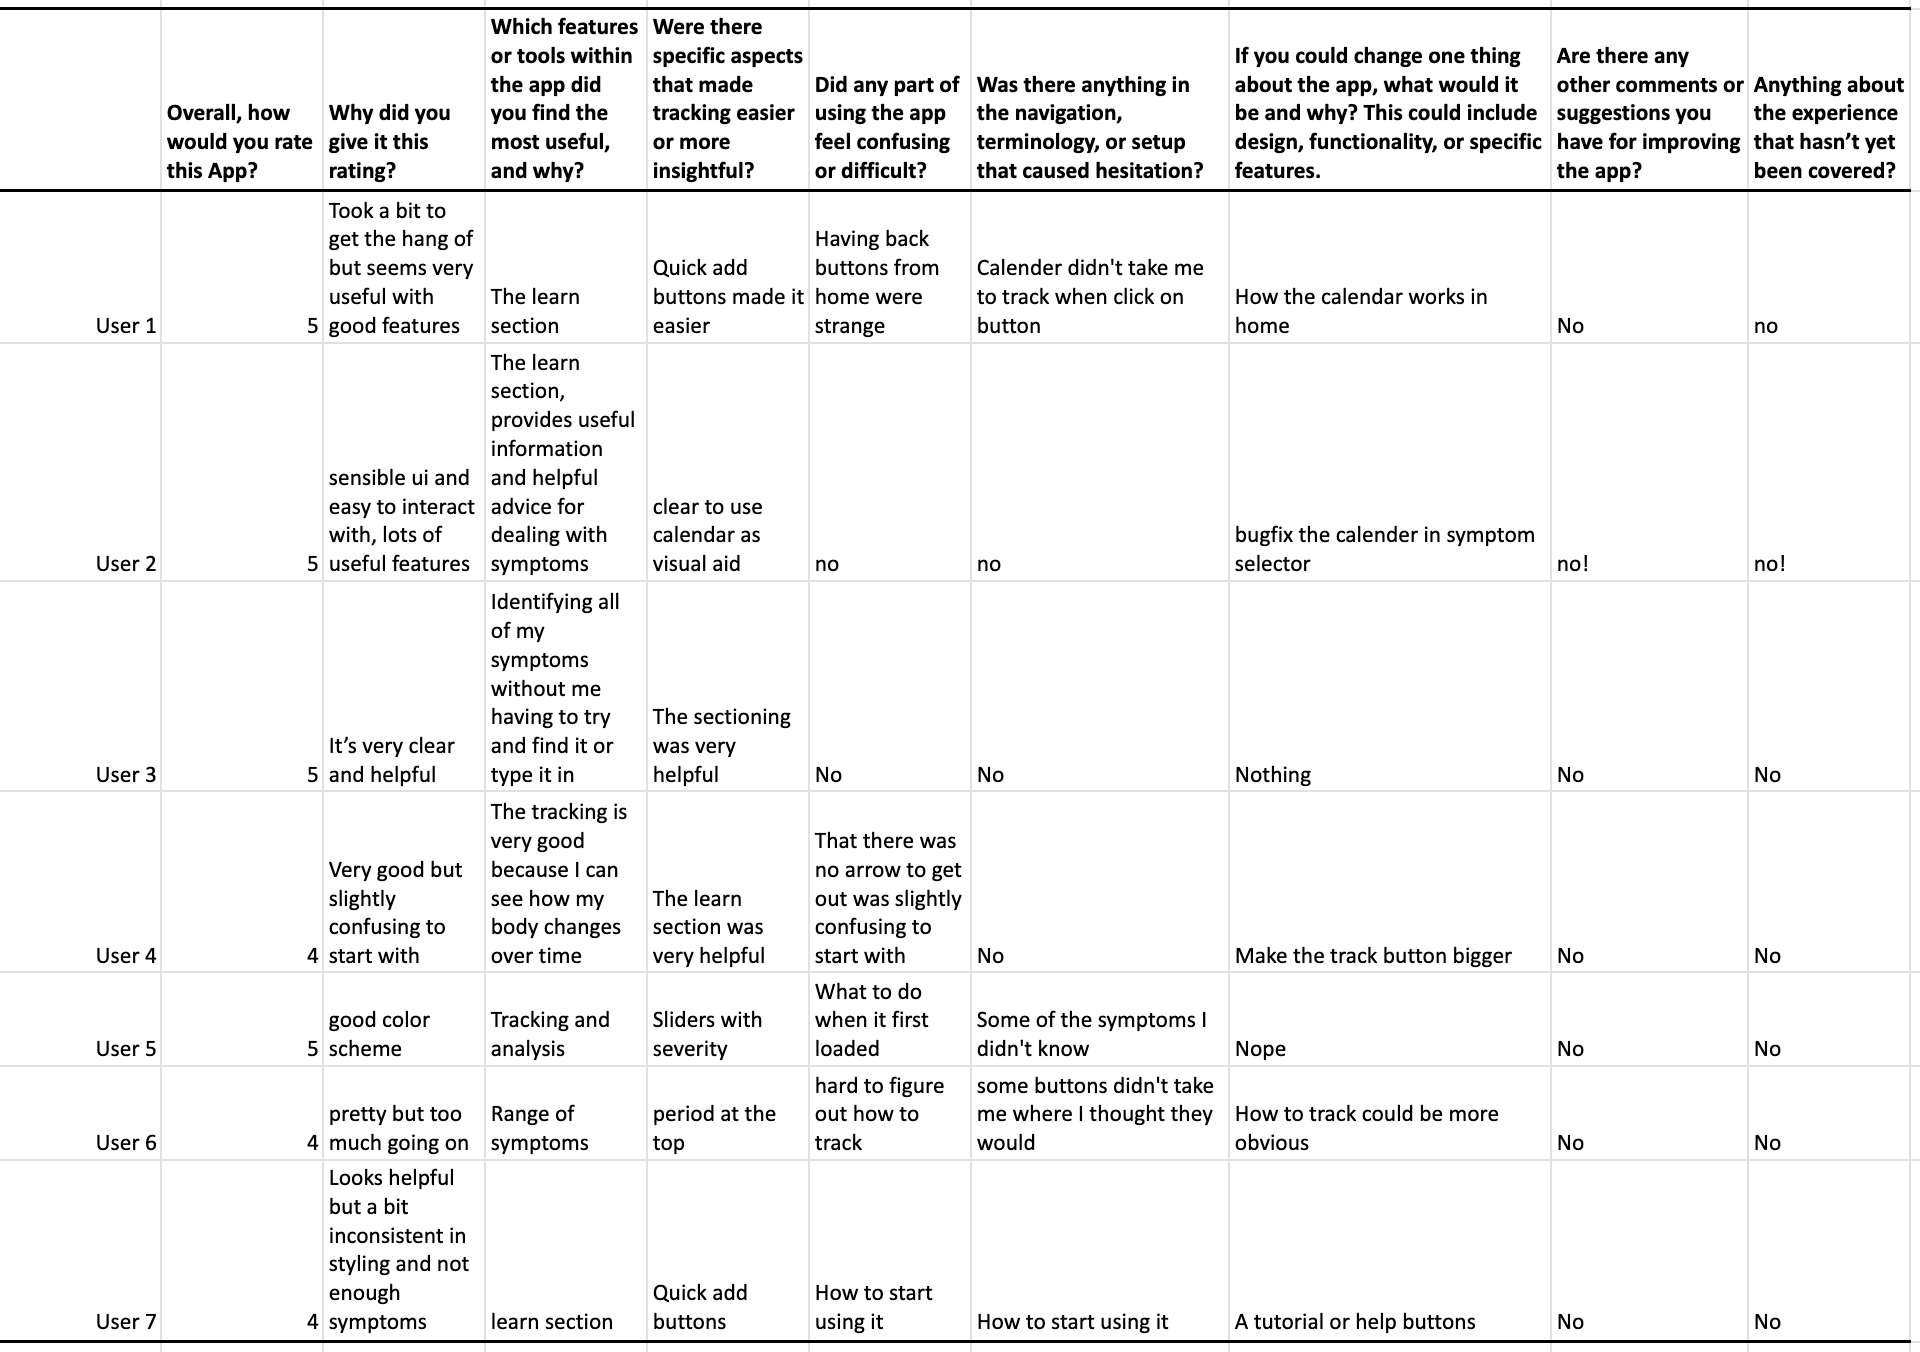
\includegraphics[scale=0.3]{GA-frq.png}
          \caption{Group A Free Response Questions Feedback}
          \label{figure:ga-frq}
        \end{center}
      \end{figure}
    

\subsubsection{Round 3: React Native Evaluation with Group B}
After implementing the feedback from Group A, the updated React Native app was then tested with a new group of 7 participants. This group was also asked to fill out a SUS and long answer questions about their experience with the app. The goal of this round of testing was to see if the changes made had a positive impact on the usability of the app.

The changes made included: 
\begin{itemize}
    \item Adding padding to the navigation bar
    \item Emphasiging the Track button through color, size, and shape
    \item Calender functionality was fixed so that when a user clicks on a day it takes them to the track page with the date preselected
    \item The calendar in Symptom Selector was fixed to allow users to change the date they are tracking data for directly in the track page wihout having to go back to the home or calendar page
    \item Fixed navigation so that the back button always appears after switching pages
    \item Greyed out future dates in the calendar so a user can't track dates in the future
    \item Added days of the week initials to the top left hand corner of the calendar day boxes in the home page
    \item Added a data reload funciton to the home page triggered by pulling down on the screen 
    \item Fixed how the symptoms that are tracked are displayed in the calendar detail view when a user clicks on a day in the big calendar
    \item Fixed the Edit button in the big calendar day detail view 
    \item Fixed the most common symptom analysis widget to correctly display the most common symptom tracked
    \item Adjusted the style of components to be more comptible with the high contrast mode 
    \item Refined the export to CSV functionality to not include data that was stored as None or empty so that only the tracked symptoms show in the CSV
\end{itemize}


\begin{table}[]
    \caption{Round 3 SUS Results for Group B React Native App}
    \label{table:grp-b-sus}
    \resizebox{\textwidth}{!}{
    \begin{tabular}{llllllll}
    \hline
    \multicolumn{8}{l}{SUS Group B Results}                                                                                                                \\ \hline
                                                                                            & User 1 & User 2 & User 3 & User 4 & User 5 & User 6 & User 7 \\
    I think that I would like to use PeriPath frequently.                                   & 5      & 5      & 5      & 5      & 5      & 5      & 5      \\
    I found PeriPath unnecessarily complex.                                                 & 2      & 2      & 1      & 1      & 2      & 1      & 1      \\
    I thought PeriPath was easy to use.                                                     & 5      & 4      & 4      & 5      & 5      & 5      & 4      \\
    I think that I would need the support of a technical person to be able to use PeriPath. & 2      & 1      & 1      & 1      & 1      & 1      & 1      \\
    I found the various functions in PeriPath were well integrated.                         & 5      & 5      & 5      & 4      & 4      & 5      & 4      \\
    I thought there was too much inconsistency in PeriPath.                                 & 2      & 1      & 2      & 2      & 1      & 1      & 1      \\
    I would imagine that most people would learn to use PeriPath very quickly.              & 4      & 5      & 5      & 5      & 5      & 3      & 5      \\
    I found PeriPath very cumbersome to use.                                                & 1      & 1      & 1      & 1      & 1      & 1      & 1      \\
    I felt very confident using PeriPath.                                                   & 4      & 5      & 5      & 5      & 5      & 5      & 5      \\
    I needed to learn a lot of things before I could get going with PeriPath.               & 3      & 1      & 1      & 2      & 1      & 2      & 1      \\ \hline
    SUS Score                                                                               & 82.5   & 95     & 95     & 92.5   & 95     & 92.5   & 95     \\
    Average SUS Score from all users                                                        & \multicolumn{7}{l}{92.5}                                     \\ \hline
    \end{tabular}
    }
    \end{table}

    As seen in Table \ref{table:grp-b-sus}, the SUS scores ranged from 82.5 to 95, with an average SUS score of 92.5, which places the app in the 92nd percentile. This indicates that the app is highly usable and meets the needs of the target audience. All participants stated that they Strongly Agree that they would like to use the app frequently and all participants strongly disagreedd with the statement that the app was very cumbersome to use. All participants also stated that they agreed or strongly agreed that they felt very confident using the app and that it was easy to use. 

    \begin{figure}[h!!]
        \begin{center}
          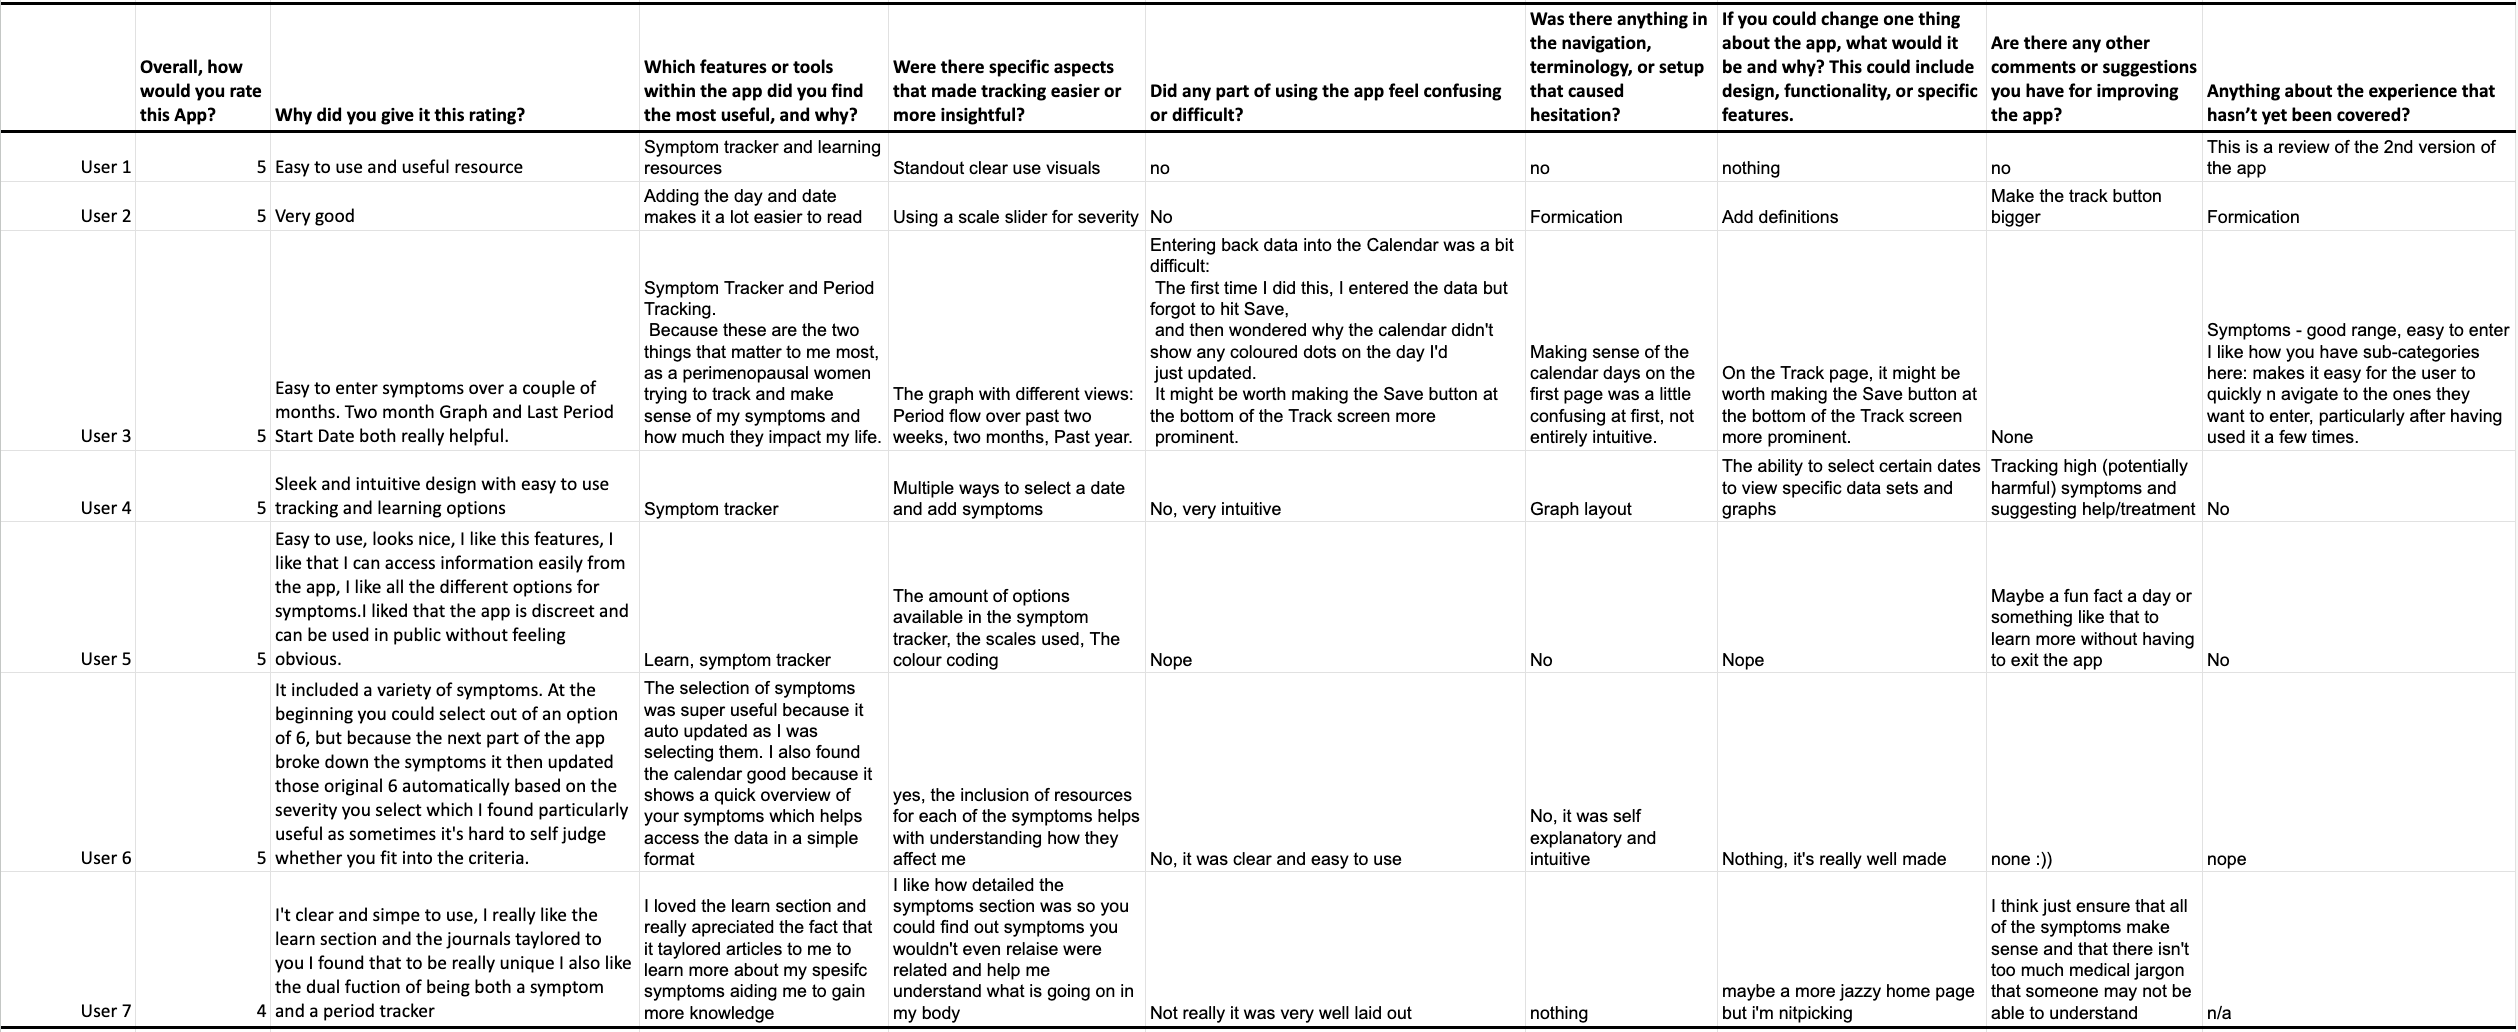
\includegraphics[scale=0.35]{GB-frq.png}
          \caption{Group B Free Response Questions Feedback}
          \label{figure:gb-frq}
        \end{center}
      \end{figure}

The feedback from the free response questions in Figure \ref{figure:gb-frq} was also very positive, with many participants noting that they would use the app again and that they found it helpful for tracking their symptoms. The average rating of the app out of 5 was 4.8 with 5 beign the highest rating. Severy users stated that information was easy to acccess and track. Many stated that they liked the variety of symptoms that could be tracked and that it was helpful to see symptom they didn't even realise were related to perimenopause to help self reflect. One user even stated that they especially liked the fact that the app was discreet looking and could be used in public without feeling obvious. Several users stated the uniqueness and dual functionality of the app being a period tracker and a symptom tracker was a big selling point.  

Improvement suggestions included:
\begin{itemize}
    \item making the track save button bigger
    \item offering help/treatment for symptoms tracked with high severity
    \item make the home page look more interesting
    \item add a fun fact a day related to perimenopause
    \item make the track button bigger
    \item make sure all the symptoms are put in terms most people would understand and are not medical jargon
\end{itemize}

\subsection{Results of Evaluation}

\subsubsection{User Requirements Results} 
From the user requirements survey, it is clear that the majority of participants are in the perimenopausal stage and experience symptoms related to this stage. The survey also revealed that many participants do not currently track their symptoms, indicating a potential need for a a potential gap and a potential need for a user-friendly tracking app that can help users monitor their symptoms and provide insights into their health. We can conclude this because the high symptom prevalence confirms the importance of addressing user needs in this demographic. A tracking app is also suitable as it would has the potential benefit of customizable or comprehensive tracking features for the diverse symptoms experienced by perimenopausal women as highlighted in the survey. 


\subsubsection{Round 1: Web App Evaluation}
The average score of 73.5 places the web app in the 73rd percentile which indicates acceptible usability but there is room for improvement. The feedback from the participants highlighted several areas for improvement, including the need for more graphs, a summary page for symptoms, and larger text size. These suggestions were taken into account when making changes to the app for the next round of testing. After researching the causes of some of the issues, it was found that the web app was not responsive and did not work well on different screen sizes. The behavior also changed slightly depending on the browser used. This was a significant issue as the app was designed to be used on mobile devices, and the lack of responsiveness made it difficult for users to navigate the app. The decision was made to switch to a React Native app, which would allow for better performance and usability on mobile devices.

\subsubsection{Round 2: React Native Evaluation with Group A}
The increase in average SUS score from the 73.5th percentile to the 82.85th percentile shows that the design changes had a significant positive impact on the usability, look, and feel of the app. Many uses stated that they would use the app again and that it was easy to use once they figured out how to track symptoms and navigate the app. The main areas for refinement were slight inconsitencies in navigation and calendar functionality however it was still much better received than the initial web app. 

\subsubsection{Round 3: React Native Evaluation with Group B}
92nd percentile, significant increase from group A results.
The changes made to the app were well received by the participants, and the feedback was overwhelmingly positive. The participants found the app easy to use and appreciated the changes made to the look and feel of the app. The average SUS score of 92.5 indicates that the app is highly usable and meets the needs of the target audience. The increase in FRQ App Rating out of 5 from 3.8 in stage 1, to 4.8 in stage 3 shows that not only is the app more usable but that the useres agree and are aware of the increase in quality of the app. The consistent top scores on ease of use, integration of functions, and reduced complexity reflect that previous issues were effectively addressed. Participants also showed high confidence and readiness to adopt the app, suggesting that the changes positively impacted the overall user experience. 

\subsubsection{MARS Evaluation}
The app was then rated according to the MARS rating system and compared to the other app rated at the beginning of the study. **Results here** 

